\section{Excess velocity at arrival}

The excess velocity at arrival is the difference between the velocity of the
spacecraft at arrival and the velocity of the interloper at arrival. The
velocity of the spacecraft at arrival is denoted by $\vec{v_{\infty ,2}}$. Note
that this velocity represents the velocity after the second impulse of Lambert's
maneuver, leading to a rendezvous with the interloper. The velocity of the
interloper at arrival is $\vec{v_\text{ISO}}$. Thus, the excess velocity at
arrival is:

\begin{equation}
    \Delta v_2 = \norm{\vec{v_{\infty ,2}} - \vec{v_\text{ISO}}}
\end{equation}


\subsection{'Oumuamua}

Porkchop plots for 1I/'Oumuamua representing the excess velocity at arrival are
shown in figure \ref{fig:oumuamua-direct-prograde-transfer-porkchop-avl} and figure
\ref{fig:oumuamua-direct-retrograde-transfer-porkchop-avl}.

\begin{figure}[H]
  \centering
  \includegraphics[width=\textwidth]{static/oumuamua/direct-prograde-transfer-porkchop-avl.png}
        \caption[Direct and prograde launch energy porkchop for 'Oumuamua]{Launch energy porkchop plot for 1I/'Oumuamua for a direct and prograde
        transfer showing the isolines for the arrival velocity required for a rendezvous.}
  \label{fig:oumuamua-direct-prograde-transfer-porkchop-avl}
\end{figure}

\begin{figure}[H]
  \centering
  \includegraphics[width=\textwidth]{static/oumuamua/direct-retrograde-transfer-porkchop-avl.png}
        \caption[Direct and prograde launch energy porkchop for
        'Oumuamua]{Launch energy porkchop plot for 1I/'Oumuamua for a direct and
        retrograde transfer showing the isolines for the arrival velocity required for a rendezvous.}
  \label{fig:oumuamua-direct-retrograde-transfer-porkchop-avl}
\end{figure}

Again, for short times of flight, the excess velocity at arrival is higher
whereas for longer times of flight, the excess velocity at arrival is lower. 

Nevertheless, the isolines for the excess velocity at arrival show an
interesting pattern. They all born in a common point. This point is located
around later 2017 and is analyzed in detail within the next section. 

Regarding comonalities between the prograde and retrograde transfers, both show
a similar pattern for the arrival velocity.

\subsection{Borisov}

Porkchop plots for 2I/Borisov representing the excess velocity at arrival are
shown in figure \ref{fig:borisov-direct-prograde-transfer-porkchop-avl} and figure
\ref{fig:borisov-direct-retrograde-transfer-porkchop-avl}.

\begin{figure}[H]
  \centering
  \includegraphics[width=\textwidth]{static/borisov/direct-prograde-transfer-porkchop-avl.png}
        \caption[Direct and prograde arrival excess velocity porkchop for
        Borisov]{Launch energy porkchop plot for 2I/Borisov for a direct and
        prograde transfer showing the isolines for excess velocity at arrival
        for a rendezvous.}
  \label{fig:borisov-direct-prograde-transfer-porkchop-avl}
\end{figure}

\begin{figure}[H]
  \centering
  \includegraphics[width=\textwidth]{static/borisov/direct-retrograde-transfer-porkchop-avl.png}
        \caption[Direct and retrograde arrival excess velocity porkchop for
        Borisov]{Launch energy porkchop plot for 2I/Borisov for a direct and
        retrograde transfer showing the isolines for excess velocity at arrival
        for a rendezvous.}
  \label{fig:borisov-direct-retrograde-transfer-porkchop-avl}
\end{figure}

Once again, the excess velocity at arrival for Borisov remembers the ones for
the case of 'Oumuamua. Again, the values are different and higher for the second
discovered interloper.

Similarly to 'Oumuamua, the lines for the arrival velocity start at a common
point. In this case, the point is located at the beginning of 2020 for launch
dates. However, the main difference with the first discovered interloper is that
a series of closed lines shows for an arrival at year 2020. These series are
analyzed in detail in the next section.
